% NeurIPS 2026 workshop submission. Replace the workshop title below and
% switch the blind-review option if required by the target workshop.
\documentclass{article}
\PassOptionsToPackage{numbers,sort&compress}{natbib}
\usepackage[dblblindworkshop]{neurips_2026}
\usepackage[utf8]{inputenc}
\usepackage[T1]{fontenc}
\usepackage{graphicx}
\usepackage{amsmath}
\usepackage{amssymb}
\usepackage{booktabs}
\usepackage{xcolor}
\usepackage{microtype}
\usepackage{url}
\usepackage[bookmarks=false,hidelinks]{hyperref}

\emergencystretch=1.5em
\renewcommand\UrlFont{\rmfamily}
\urlstyle{rm}

\workshoptitle{NeurIPS 2026 Workshop on Interpretability for Discovery}
\title{From Readable to Causal: Testing Sparse Autoencoder Features in Agent Tool Selection}

% The double-blind workshop style suppresses this block for review.
\author{%
  Hannes Hapke \\
  575 Lab, Dataiku Inc.\\
  Portland, OR, USA\\
  \texttt{hannes.hapke@dataiku.com}
  \And
  David Cardozo \\
  575 Lab, Dataiku Inc.\\
  Toronto, ON, Canada\\
  \texttt{david.cardozo@dataiku.com}
}

\begin{document}
\maketitle

\begin{abstract}
Sparse autoencoders (SAEs) expose readable features in language-model
activations, but readability does not establish causation. We test this gap in
agent tool selection by ablating and cross-patching JumpReLU SAE features at
the decision token without changing the prompt. Small cue-feature sets can
redirect tool choice at natural activation scales, including one
single-feature case, but reproduce only part of a full-state residual patch
and show no observed advantage over an equal-magnitude dense direction. The sparse basis thus
offers nameable rather than uniquely effective control. In this model, causal
leverage concentrates in late evaluated layers even though earlier features
describe the relevant cues. We also find a nearly collapsed dictionary with
the study's strongest reconstruction but no usable contrastive structure.
Cue patches reproduce part of the full-state reference on two small, curated
distribution-shift probes. These results place input-specific dictionary health
before feature meaning or causal coverage, with conclusions local to the
tested model and closed-set task.
\end{abstract}

\section{Introduction}
\label{sec:intro}

When an agent selects a tool, an SAE can identify features that co-vary with
the request and attach readable labels to them
\citep{ref_bricken2023,cunningham2023sparseautoencodershighlyinterpretable}.
That is descriptive evidence, not yet an explanation. A feature may help
determine the tool, or merely read out a cue or a decision represented
elsewhere. The distinction matters whenever a feature dashboard is interpreted
causally or used as a steering interface.

We study this gap with interventions in the SAE basis. Minimal request pairs
differ by a controlled cue and produce different tools. At the token where the
model emits its choice, we remove one side's cue features or transplant the
other side's values while leaving the recipient prompt unchanged. This is
activation patching
\citep{meng2022locatingeditingfactualassociations,
wang2022interpretabilitywildcircuitindirect} at a sparse, nameable interface,
with mass- and difference-matched controls. Unlike work that starts from a
behaviorally chosen steering direction
\citep{turner2024steeringlanguagemodelsactivation,templeton2024scaling}, we ask
whether features from an existing SAE form a faithful causal decomposition.
Prior evaluations likewise caution that reconstruction and sparsity need not
predict interpretability or steering utility
\citep{gao2024scalingevaluatingsparseautoencoders,
makelov2024principledevaluationssparseautoencoders}.

Three results qualify one another. First, small cue-feature sets can redirect
tool choice, and one feature redirects one evaluated direction. Second, a full
residual patch supplies the missing denominator: cue features reproduce 29\% of
its flips, with no observed advantage over a dense direction of equal
magnitude. The SAE basis therefore provides a causal intervention that can be
named, but not one observed here to control more of the decision. Third, readable features
are almost inert at early layers, and one high-reconstruction dictionary
collapses on the evaluated inputs. The contribution is consequently not a
universal steering mechanism, but an evaluation discipline: check the
dictionary's input-specific structure first; then test feature specificity,
compare against a full-state reference and dense alternatives, and audit
where and how the intervention acts.

\section{Causal evaluation}
\label{sec:method}

\paragraph{Model and decision.}
We evaluate NVIDIA Nemotron-3.5-Nano-30B-A3B in BF16, a 52-layer hybrid of
Mamba-2, attention, and mixture-of-experts blocks with residual width 2,688
\citep{nvidia2026nemotron35}.
Released JumpReLU SAEs \citep{ref_rajamanoharan2024} cover layers
$\{6,13,20,27,34,43\}$ at the residual entering each layer, have 10,752
features, and target $L_0=75$. They were trained, without contrastive
supervision, on decision-token activations from the same generated corpus the
in-distribution evaluation draws on: the 1,574,523 of 2,011,672 generated
pairs whose two sides call different tools. 136 of the 150 unique demonstration and expanded requests occur in
it verbatim, and the second draw's 128 (Sect.~\ref{sec:limitations}) come from
the same sweep.
Each prompt lists six tools and ends with the prefill \texttt{I'll use the}.
We read the next-token tool distribution through a prefix tree and intervene
additively, preserving the residual and adding decoder deltas for an edited set
$S$: $x'=x+s\sum_{i\in S}(t_i-a_i(x))W_{\mathrm{dec},i}$, where $a_i$ is the
current activation, $t_i$ the target (zero for ablation) and $s$ the
dictionary's input scale. No reconstruction error enters the forward pass. Capture and intervention backends
agree on every expanded baseline choice; mean residual cosine is 0.999 and
0.998 by scenario, minimum 0.987.
\footnote{Anonymized code, pair definitions, run artifacts, and regeneration
scripts are available at
\url{https://anonymous.4open.science/r/ml-inspector-0651/}.}

\paragraph{Pairs and interventions.}
We sweep 377,626 supply-chain and 327,988 customer-support pairs and apply
fixed gates: both sides choose different tools at probability $\geq0.6$ with
the weaker side $<0.8$; the tool prefix tree covers $\geq0.5$ of the
decision-token mass on both sides; content-word Jaccard is at least 0.70 for
supply chain and 0.55 for customer support; no tool is named; and contrast/tool
duplication is capped. This gives four and six demonstration
pairs, alongside seven pairs from prior work \citep{ref_hapke2025}. For the
expanded study, we sample 32 pairs per main scenario with at most ten per
contrast type. These counts average over the contrast quota and are not
population prevalence estimates.

Per side we take every feature activating more strongly than on the other
side, rank by that difference, merge features whose labels---LLM annotations
from maximally activating examples, not ground truth (Appendix)---have
a normalized label-token Jaccard of at least 0.6, and keep the top six families. Selection is thus pair-adaptive and
recomputed per side; cue sets contain 3--14 features.
\textbf{Ablation} zeros the ablated side's cue features.
\textbf{Cue cross-patching} clamps donor cue values into the recipient while
its prompt remains unchanged. \textbf{Bulk cross-patching} clamps every
donor-active feature; on a dense code this becomes a representation transplant,
not sparse-feature evidence. A \emph{directed flip} changes the argmax to the
paired side's tool; third-tool changes are tracked separately.

\paragraph{Comparators and uncertainty.}
Random sets are drawn from the donor-active features outside the cue set for
cross-patching, clamped at their donor values, and from the ablated side for
ablation. They are matched on feature count and activation mass, three draws
each; a set's \emph{band} is the largest absolute effect among its draws. A
stricter family matches
$\sum_i|v_i^A-v_i^B|$, because cue features are selected precisely for
differing across the pair. If the remaining pool cannot reach the target, we
use the whole pool and label it a ceiling rather than a match. We also use
three dictionary-free references: patching the full donor residual at the
decision token, a contrast-level mean residual direction computed without the
current pair, and random residual directions. The dense direction is evaluated
both at the full donor--recipient norm and at the smaller norm of the cue
clamp.

Expanded pairs are near-duplicates within a contrast and both directions are
dependent, so we report exact dependent counts. We resample whole
scenario-by-contrast clusters, retaining every observation in a drawn cluster
and drawing within scenario, and enumerate the resampling distribution exactly
rather than sampling it, weighting each count vector by its multiplicity
(Appendix). Clusters are unequal in size, so this fixes how many clusters each
scenario contributes, not how many pairs. With so few clusters these percentile
brackets are
uncalibrated and likely to understate uncertainty, not nominal 95\%
intervals. We do not attach tests that treat intervention rows as independent.

\section{Results: a health-first audit}
\label{sec:results}

\paragraph{Health-first validation.}
Feature-level patching requires input-specific dictionary structure. The
layer-43 anomaly motivated a retrospective audit of each scenario--layer cell
on per-prompt $L_0$, always-on share, and median side-specific count; explained
variance and $L_0$ alone are insufficient. We therefore exclude customer support at layer
43 despite its highest explained variance, so those bulk flips are not
feature-level evidence (Sect.~\ref{sec:collapse}). We report it as exploratory, not a
prespecified rule. Remaining cells proceed through matched controls, a
full-state reference and dense comparator, then localization, semantic, and
generation checks.

\subsection{After the health screen: partial causal coverage}
\label{sec:coverage}

Our clearest healthy-cell case is a supply-chain pair differing only by \emph{forecasted}. At layer 43,
cross-patching feature 2101 (\emph{safety stock and inventory coverage
calculation}) into the unmodified request changes \texttt{demand\_forecaster}
to \texttt{inventory\_manager}, raising the latter from 0.15 to 0.71 at the
donor's natural activation; all six cue families reach 0.73 and mass-matched
random sets move it by at most 0.05. This establishes existence, not typicality.

On the expanded sample, cue cross-patching redirects 29 of 128 directions to
the donor tool and 3 to a third. Bulk
patching redirects 41. Matched at the same family level, control draws flip 15
times in 2,289 against 23 in 763 cue families. Cue ablation changes 81 of 128 argmaxes: 68 to the
paired tool and 13 elsewhere. Its destination is confounded: all 63 flips on
runner-up sides are directed, against 5 of 18 elsewhere (Appendix
Table~\ref{tab:runnerup}). Cue ablation exceeds the stricter
difference-matched comparison on 57 of 63 genuine matches and 60 of 65 pool
ceilings; one matched side flips without beating its control
band, and we exclude it as evidence. These comparisons are descriptive because
their rows remain clustered.

Flip counts need a denominator. A full residual donor patch redirects 100 of
128 directions (Table~\ref{tab:ceiling}): a full-state reference rather than a
bound, since bulk patches flip 2 directions where it does not. The cue flip
ratio is $29/100=0.29$ and the bulk ratio 0.41. A contrast-level dense
direction matched to the cue clamp's norm redirects 30 of 124 against the cue
set's 28, and equal-norm random directions never redirect
(Table~\ref{tab:ceiling}). The arms disagree on 14 directions; a
scenario-stratified cluster resampling puts the difference at $-1.6$ pp,
uncalibrated bracket $[-7.0,+7.6]$, not an equivalence test
(Appendix Table~\ref{tab:discordance}). For this contrast-mean direction the larger
norm produces more redirects, and the equal-norm comparison shows no observed
sparse-basis advantage. Given an already trained and labeled SAE, cue selection
needs only the current pair while the dense direction needs sibling pairs from
the same contrast; we do not compare end-to-end data or compute.

\begin{table}[t]
\caption{Decision-token interventions on the expanded sample, ordered by
directed flips. The \emph{reference-normalized flip ratio} is directed flips
over the 100 of the full-state reference.
Difference-in-means is unavailable for four directions with no other pair of
the same contrast. Brackets on the cue row give its count on the same 124
directions. Counts are dependent, not independent trials.}
\label{tab:ceiling}
\centering
\small
\setlength{\tabcolsep}{5pt}
\begin{tabular}{@{}llcc@{}}
\toprule
Intervention & Basis & Directed flips & Flip ratio \\
\midrule
Full residual patch              & model & 100/128 & 1.00 \\
Difference-in-means, full norm   & model & 79/124  & --- \\
All donor-active features        & SAE   & 41/128  & 0.41 \\
Difference-in-means, clamp norm  & model & 30/124  & --- \\
Cue features                     & SAE   & 29/128 [28/124] & 0.29 \\
Random direction, clamp norm     & model & 0/372   & --- \\
\bottomrule
\end{tabular}
\end{table}

The reference also changes the scenario comparison. Supply chain has more cue
flips than customer support (16/64 versus 13/64), but its full residual patch
redirects 61/64 directions while customer support redirects only 39/64.
Against their respective references the cue flip ratios are therefore 0.26 for
supply chain and 0.33 for customer support.
On the 25 customer-support directions where even a full patch does not cross
the argmax, the donor probability can still move substantially (from 0.04 to
0.47 in one case), suggesting the recipient context partly re-derives the
decision downstream.

In the small arm where generation is tested:
five of twenty decision-position interventions first flip the next-token
argmax, and all five then name the donor tool in 48 generated tokens; none of
twenty difference-matched controls does. Five events establish little beyond
the first action. On authored contrast types absent from SAE training, all
seven cue redirects fall among the 25 full-state-reference redirects of 30
directions and span five of the six represented axes. On a separate released
tool-selection split both cue redirects fall among thirteen reference
redirects, from two of seven pairs. These are exact dependent counts on curated
probes, not population rates; the second also changes scenario and dictionary
density (Appendix).

\subsection{Readable cues have little early-layer leverage in this model}
\label{sec:depth}

Across layers 6, 13, and 20, 1 of 460 interventions produces a directed flip.
At the selected primary layers 137 of 324 flip, against 38 of 324 at the
unselected layer 27, where the expanded sample gives 20/128 ablation and 15/128
cross-patch. The contrast is not merely an argmax effect: against random sets matched
on how much they differ across each pair, the median cue/control effect ratio
is $0.81\times$ at layers 6--20 and $2.81\times$ at layers 27--43, with cue
sets clearing their bands on 21/59 early versus 54/68 late sides. Denominators
count difference-matched sides with a finite band; ceiling draws and 16
zero-band sides are excluded.

Early SAEs nevertheless contain readable features that separate the pair
sides, including those reported in our earlier layer-20 analysis
\citep{ref_hapke2025}. Position interventions rule out a simple mismatch:
at the primary layer, decision-position ablation changes 15/20 tools while
request-token and all-but-decision ablation change no argmax, though
probabilities do move (max $|\Delta p|$ 0.03 and 0.24); at layer 20, no
position set changes any of the 20 tools. Thus readability and causal leverage
separate on this evaluated model--task grid. Layers 34 and 43 are the most
responsive of six tested.

\subsection{Causal does not mean semantically general}
\label{sec:semantics}

Cross-patching establishes that a feature affects the choice, not what it
represents. Keyword probes insert a cue word into the paired request in a
semantically inert role; 9 of 12 preserve the expected tool. Paraphrases remove
the cue word while keeping its meaning; 30 of 40 preserve the behavior.
Inserting \emph{forecasted} only as a modifier of budget codes leaves the tool
unchanged. These probes bound behavior, not feature content: across the 40
paraphrases the cue families keep firing in 229 of 240 family--paraphrase
evaluations, whether or not the tool holds. The cue is therefore more than a
token detector, but these probes do not identify what it encodes.

Steering is also directional. A local-to-global sourcing patch redirects the
tool at the donor's natural activation, whereas the reverse fails even at
$3\times$; urgent-versus-routine shows the opposite asymmetry. The observed asymmetry is
consistent with cue features adding evidence for a tool rather than acting as
symmetric switches, so both directions belong to the causal claim.

\subsection{Why the health screen is necessary}
\label{sec:collapse}

We return to the customer-support layer-43 cell excluded by the input-side
audit. It initially appears strongest, bulk patching redirecting 9 of 12
directions, but its SAE is nearly collapsed on these prompts: a mean of 1,167
features fires per prompt, 1,162 on every prompt, and the median pair retains
one side-specific feature. Eight of the nine flips
require transplanting all roughly 1,163 donor-active features; only one comes
from the cue families. Because the intervention adds decoder deltas rather than
replacing the state, this is a near-complete transplant of the SAE code.

Explained variance is 0.86, the highest in the study
(Fig.~\ref{fig:collapse}); raw $L_0$ is also insufficient because the same
layer-43 dictionary remains usable on tool-selection prompts despite mean
$L_0=374$. Two input-side checks detect what density misses: the always-on
share is 0.97 in the collapsed cell versus at most 0.42 elsewhere, and the
median side-specific count is 1 versus 5--69. Both precede any intervention. Across the six cells where the bulk-patch/cue-ablation
discrepancy is defined, all five non-collapsed values lie between 0.43 and
2.00, while the collapsed cell is 9.0. The arms differ: cue-only cross-patching
is 1/12 there, matching its 1/12 ablation, so the whole discrepancy is the bulk
patch. For comparison we use only the three cells with roughly three or
more ablation flips. With one ablation flip behind it, the discrepancy is an
alert corroborated by the input-side statistics, not standalone evidence.

\begin{figure}[t]
\centering
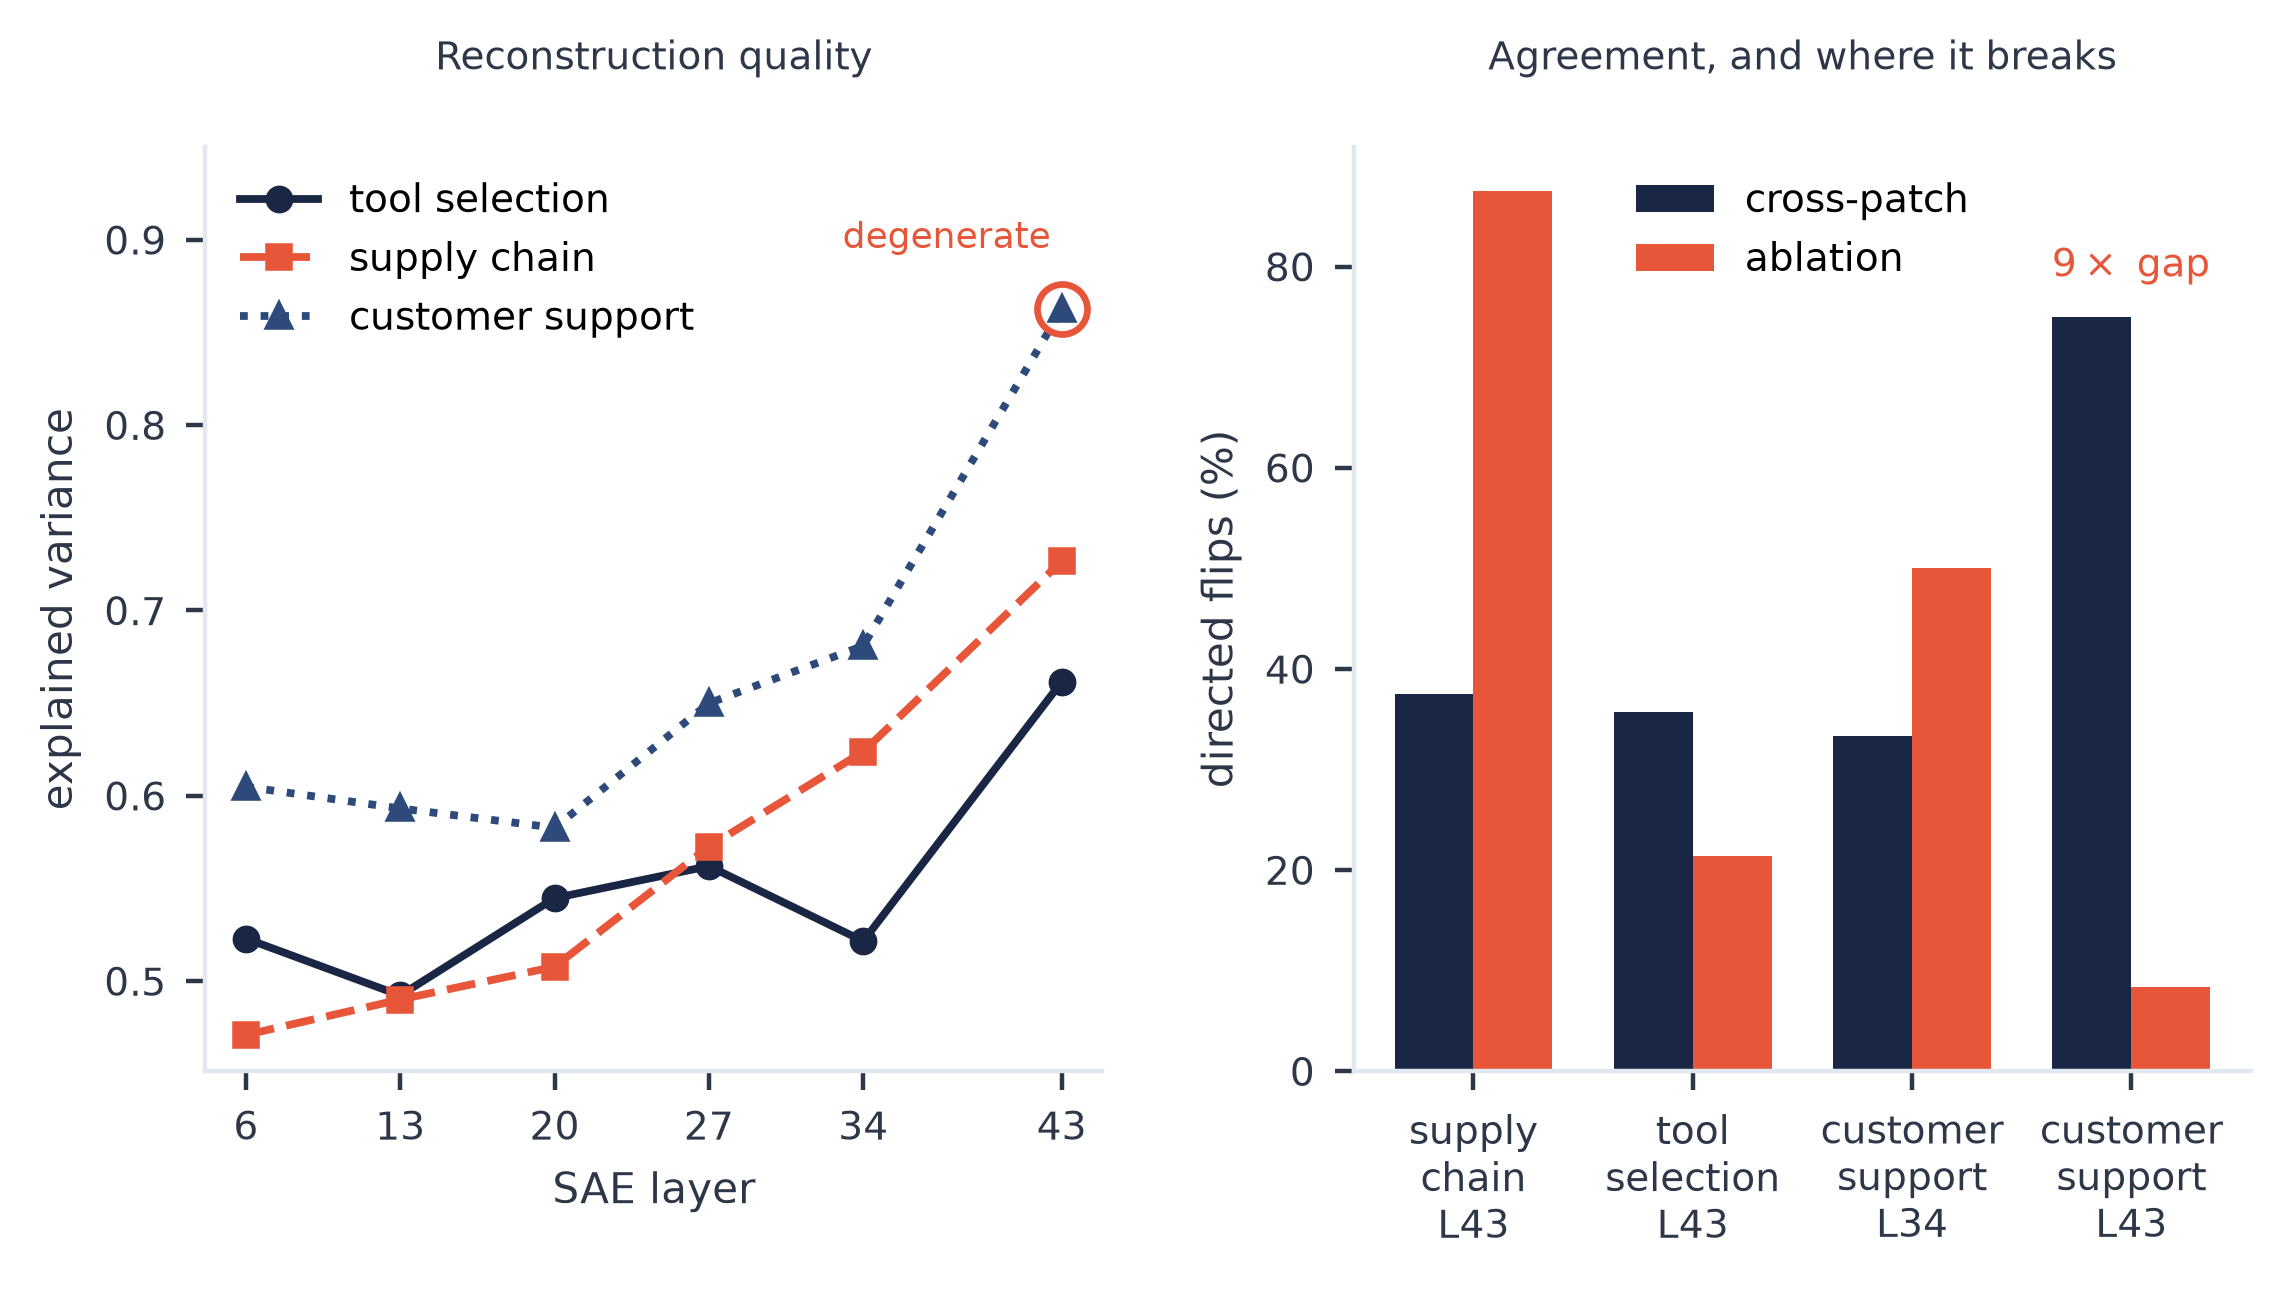
\includegraphics[width=0.94\textwidth]{images/chart_degeneracy.png}
\caption{Left: explained variance peaks for the collapsed customer-support
cell at layer 43. Right: bulk cross-patch against cue ablation, 3/8 vs.\ 7/8,
5/14 vs.\ 3/14 and 4/12 vs.\ 6/12 in the non-collapsed cells against 9/12
vs.\ 1/12 in the collapsed one, whose $9\times$ rests on one ablation event.}
\label{fig:collapse}
\end{figure}

\section{Limitations and implications}
\label{sec:limitations}

External validity is the primary limitation: one SAE release for one 52-layer
hybrid, with expanded counts in only two scenarios. The main evaluation
overlaps SAE training---136 of 150 unique demonstration and expanded requests
occur verbatim---while the authored held-out probe is not a sampled deployment
distribution. The only non-authored out-of-distribution reference gives a
lower ratio on thirteen reference flips. Replication across architectures, objectives,
scales, and open-ended actions is needed before treating
late-layer localization, the 0.29 flip ratio, or the collapse screens as
general.

\paragraph{Architecture-specific hypotheses.}
The hybrid offers an alternative to a universal late-decision story. Each SAE
site is a post-attention/pre-MoE seam in the released block pattern
\citep{nvidia2026nemotron35}, so each patch meets a router activating six of
128 experts and a readable cue may stay route-specific; between seams Mamba-2
carries or forgets recurrent state across positions
\citep{gu2023mamba,dao2024transformersssms}, and a decision-token edit leaves
earlier context intact for downstream state to buffer. Late leverage may
therefore mark convergence, not first use. Neither request-token nor
all-but-decision ablation moves an argmax, but that does not separate
buffering, routing, and convergence. Testing requires state patching, router
logs, and pre/post-block interventions.

Internal uncertainty is substantial: the expanded pairs span ten clusters and
contain near-duplicates, and the bootstrap brackets for selected-layer ablation
and bulk cross-patch, 0.42--0.66 and 0.16--0.48, likely under-cover. The contrast quota changes the estimand, and selecting primary
layers on the demonstration grid inflates their counts. The second draw preserves the depth
ordering but varies materially (Appendix), so we do not pool it.

Cue families are pairwise-difference selections, not circuits; we do not
identify their writers or readers, and label merging shapes them;
sensitivity to annotations and to the merge and cap thresholds is untested. Difference matching helps, but 65/128 sides
have no comparably different active set. Generation covers five first-tool
flips. The reference is local, and we observe no SAE advantage over
equal-norm dense steering. The claim is therefore narrow: some nameable SAE coordinates
causally control part of these decisions.

\section{Conclusion}

SAE explanations require an ordered audit. Dictionary health comes first: at
customer support layer 43, strong reconstruction and bulk-patch flips reflect a
transplant of the SAE code, not a feature-level mechanism. In healthy cells,
late-layer cue sets provide nameable but partial control and show no observed
advantage over an equal-norm dense direction. Matched controls, full-state
references, and layer, position, semantic, and generation checks should
follow. In the healthy evaluated cells, SAE features provide auditable causal
handles, not complete accounts of where decisions are made.

% The workshop limit applies to the self-contained main text above. References
% and the optional appendix begin on a fresh page and do not count.
\clearpage
\bibliographystyle{plainnat}
\bibliography{references,steering_refs}

\clearpage
\appendix

\section{Supplementary results}

\subsection{Expanded outcomes and layer comparison}

Table~\ref{tab:outcomes} records every expanded-sample outcome and
Table~\ref{tab:runnerup} splits the ablation flips by runner-up status.
Directedness is carried almost entirely by that ranking, which motivates
interpreting ablation through whether a decision changes relative to controls,
not through its destination alone. The five directed flips on sides where the
paired tool was not the runner-up are the part the ranking does not explain.

\begin{table}[h]
\caption{Full expanded-sample outcome partition. Control rows pool every
stored draw across the three matching families on the same prompts; 2,289 of
them are matched to a single cue family and are therefore smaller interventions
than a whole cue set, so the pooled rate is not comparable to the 128 cue-set
rows above.}
\label{tab:outcomes}
\centering
\small
\setlength{\tabcolsep}{6pt}
\begin{tabular}{@{}lrrrr@{}}
\toprule
Intervention & $n$ & unchanged & directed & third tool \\
\midrule
Ablation (cue families)       & 128    & 47    & 68 & 13 \\
Cross-patch (cue)             & 128    & 96    & 29 & 3 \\
Cross-patch (bulk)            & 128    & 83    & 41 & 4 \\
Ablation controls             & 3,057  & 3,032 & 6  & 19 \\
Cross-patch controls          & 3,057  & 3,015 & 27 & 15 \\
\bottomrule
\end{tabular}
\end{table}

\begin{table}[h]
\caption{Ablation flips partitioned by whether the paired tool was already the
baseline runner-up. Every flip on a runner-up side is directed, against 5 of 18
elsewhere; 75 of the 81 flips land on the baseline runner-up whichever tool
that is. Counts are dependent, so we report them without a test.}
\label{tab:runnerup}
\centering
\small
\setlength{\tabcolsep}{6pt}
\begin{tabular}{@{}lrrrr@{}}
\toprule
Paired tool is runner-up & sides & unchanged & directed & third tool \\
\midrule
Yes & 91  & 28 & 63 & 0  \\
No  & 37  & 19 & 5  & 13 \\
\midrule
All & 128 & 47 & 68 & 13 \\
\bottomrule
\end{tabular}
\end{table}

\begin{table}[h]
\caption{Cue against equal-norm difference-in-means on the 124 expanded
directions where the dense direction is defined. The comparison rests on the 14
discordant directions. Scenario-stratified whole-cluster resampling draws the
four represented contrast clusters within each scenario with replacement,
retaining all directions and both paired outcomes. For each exact distribution we enumerate all
cluster-count vectors and weight each by its multinomial probability,
equivalently enumerating every ordered draw; with $35^2=1{,}225$ vectors here
the endpoints carry no Monte-Carlo error: the cue-minus-dense
difference is $-1.6$ percentage points with 2.5--97.5 percentile endpoints of
$[-7.03,+7.63]$. Enumerating the 6,435 vectors that draw all eight clusters
together instead gives $[-7.55,+7.14]$. Because clusters are unequal in size,
drawing four per scenario does not fix how many directions each scenario
contributes; averaging the two scenario differences with equal weights, which
does, gives $[-6.71,+10.53]$ --- the upper endpoint is sensitive to that
choice, the sign of the point estimate is not. With four clusters per scenario
these are uncalibrated sensitivity brackets likely to understate uncertainty,
like those in Sect.~\ref{sec:method}, not calibrated intervals or equivalence
tests.}
\label{tab:discordance}
\centering
\small
\setlength{\tabcolsep}{6pt}
\begin{tabular}{@{}lrrr@{}}
\toprule
 & dense redirects & dense does not & total \\
\midrule
Cue redirects        & 22 & 6  & 28  \\
Cue does not         & 8  & 88 & 96  \\
\midrule
Total                & 30 & 94 & 124 \\
\bottomrule
\end{tabular}
\end{table}

\begin{table}[h]
\caption{Directed flips for the same expanded pairs at an early layer, an
unselected late layer, and each scenario's selected primary layer. The
cross-patch split is cue-only plus bulk-required flips.}
\label{tab:expanded}
\centering
\small
\setlength{\tabcolsep}{5pt}
\begin{tabular}{@{}llcc@{}}
\toprule
Scenario & Layer & Ablation & Cross-patch \\
\midrule
Supply chain     & 13          & 0/64  & 0/64 \\
                 & 27          & 11/64 & 6/64 (4+2) \\
                 & 43 selected & 40/64 & 23/64 (16+7) \\
\addlinespace
Customer support & 13          & 1/64  & 0/64 \\
                 & 27          & 9/64  & 9/64 (6+3) \\
                 & 34 selected & 28/64 & 18/64 (13+5) \\
\bottomrule
\end{tabular}
\end{table}

\paragraph{Sampling sensitivity.}
The contrast quota changes the estimand: \emph{cost vs.\ speed} supplies 0/20
cue cross-patch flips while occupying ten sampled pairs despite comprising only
3\% of the gated supply-chain population. A second 32-pair draw per scenario
gives 69/128 ablation and 33/128 bulk cross-patch changes, versus 68 and 41 in
the reported draw. Because it was sampled after the first analysis, we report
it as a sensitivity check rather than pool it.

\subsection{Full demonstration depth grid}

Each entry in Table~\ref{tab:depth-full} is cross-patch directions followed by
ablation sides. The starred customer-support cell is the collapsed dictionary
discussed in Sect.~\ref{sec:collapse}.

\begin{table}[h]
\caption{Directed flips at every evaluated SAE layer.}
\label{tab:depth-full}
\centering
\small
\setlength{\tabcolsep}{7pt}
\begin{tabular}{@{}lccc@{}}
\toprule
Layer & Tool selection (7 pairs) & Supply chain (4 pairs) & Customer support (6 pairs) \\
\midrule
6  & 0/14 $\cdot$ 0/14 & 0/8 $\cdot$ 0/8 & 0/12 $\cdot$ 0/12 \\
13 & 0/14 $\cdot$ 0/14 & 0/8 $\cdot$ 0/8 & 0/12 $\cdot$ 0/12 \\
20 & 0/14 $\cdot$ 0/14 & 0/8 $\cdot$ 0/8 & 0/12 $\cdot$ 0/12 \\
27 & 1/14 $\cdot$ 0/14 & 0/8 $\cdot$ 0/8 & 1/12 $\cdot$ 1/12 \\
34 & 2/14 $\cdot$ 0/14 & 2/8 $\cdot$ 1/8 & \textbf{4/12 $\cdot$ 6/12} \\
43 & \textbf{5/14 $\cdot$ 3/14} & \textbf{3/8 $\cdot$ 7/8} & 9/12$^\star$ $\cdot$ 1/12 \\
\bottomrule
\end{tabular}
\end{table}

\subsection{Natural-scale single-feature case}

\begin{figure}[h]
\centering
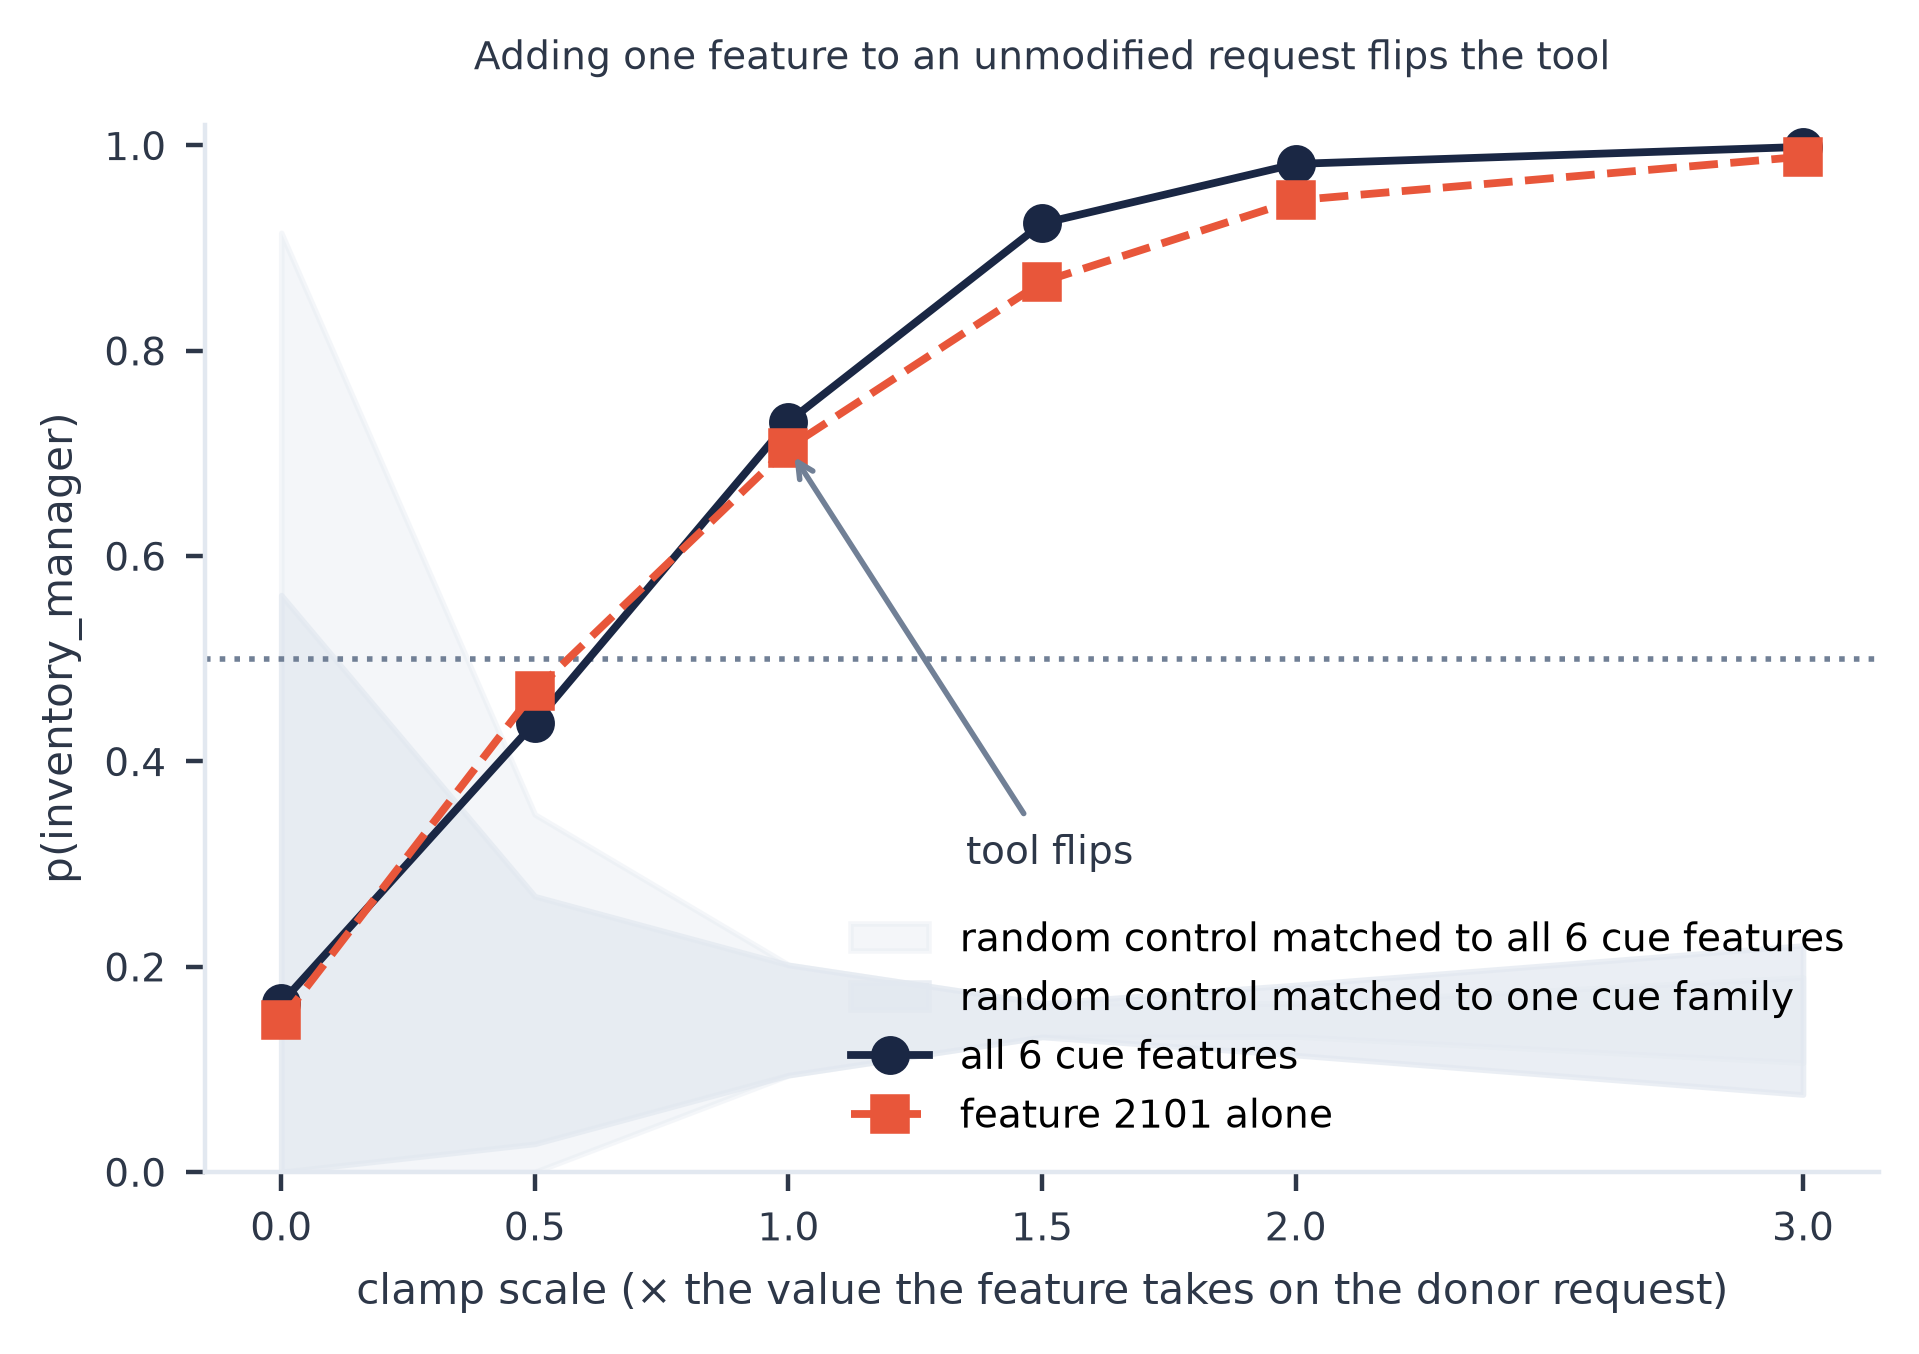
\includegraphics[width=0.84\textwidth]{images/chart_dose.png}
\caption{Cross-patching feature 2101 into the unmodified recipient request.
The tool boundary is crossed at the donor's natural activation. Shading is the
largest deviation from three random sets matched to the feature (dark) or the
whole cue set (light).}
\label{fig:dose}
\end{figure}

\clearpage
\subsection{Dictionary health}

\begin{table}[h]
\caption{Health of the deepest evaluated dictionaries. Always-on counts
include their share of the active code in parentheses; side-specific is the
median count active on one side of a pair and not the other.}
\label{tab:health}
\centering
\small
\setlength{\tabcolsep}{5pt}
\begin{tabular}{@{}llrrrr@{}}
\toprule
Scenario & Layer & Mean $L_0$ & Expl.\ var. & Always on & Side-specific \\
\midrule
Supply chain     & 34 & 36  & 0.62 & 2 (0.01)     & 18 \\
Supply chain     & 43 & 32  & 0.73 & 16 (0.18)    & 5 \\
Tool selection   & 34 & 633 & 0.52 & 222 (0.20)   & 69 \\
Tool selection   & 43 & 374 & 0.66 & 219 (0.42)   & 22 \\
Customer support & 34 & 73  & 0.68 & 42 (0.19)    & 13 \\
Customer support & 43 & 1,167 & 0.86 & 1,162 (0.97) & 1 \\
\bottomrule
\end{tabular}
\end{table}

\subsection{Compute resources}

Reported captures and interventions used one 80\,GB NVIDIA H100: about two
minutes per scenario for capture and three minutes for a one-layer battery of
128 interventions plus matched controls, under two GPU-hours total. The
preceding behavioral sweep and SAE training required substantially more compute
and are excluded from that total.

\subsection{Weights and revisions}

Hugging Face resolves \texttt{main} unless a revision is given, so naming a
repository does not identify the weights a rerun will load. All results here
use SAE repository
\texttt{575-lab/kiji-inspector-NVIDIA-Nemotron-3.5-Lightning-30B-A3B-BF16} at
commit \texttt{2380c95c}, and base checkpoint
\texttt{nvidia/NVIDIA-Nemotron-3.5-Nano-30B-A3B-BF16} at commit
\texttt{d468880b} --- the same weights the dictionaries were fitted on, which
the SAE model card records under the pre-release name
\texttt{ga\_nvidia\_nemotron\_3\_5\_nano\_bf16\_07292026\_vv0.1} at code revision
\texttt{65ae86b}. The distinction is not hypothetical: upstream \texttt{main}
has since moved past the base commit we used. The SAE loader now sends its
pinned revision by default; the base checkpoint is passed as a local
directory, so it is pinned by fetching that revision explicitly
(\texttt{hf download \ldots{} --revision d468880b}) before stripping the
draft stack. We run the base checkpoint with its multi-token
prediction draft stack removed, which rewrites only the config and the shard
index and hardlinks every weight shard, so the shards carry upstream's own
checksums. SHA-256 for all six SAE checkpoints and all 27 base-checkpoint
files are released with the run artifacts.

\subsection{Licenses}

The NVIDIA Nemotron-3.5-Nano-30B-A3B-BF16 checkpoint uses the OpenMDW License
Agreement 1.1; Qwen's Qwen3-VL-235B-A22B-Instruct-FP8 uses Apache-2.0.
The released SAE checkpoints, labels, reports, code, pair definitions, run
artifacts and regeneration scripts use Apache-2.0.
PyTorch uses BSD-3-Clause (its binaries include separately licensed
components); Hugging Face Transformers and vLLM use Apache-2.0.

\subsection{Feature labels}

The SAE release generated labels with Qwen3-VL-235B-A22B-Instruct-FP8 from
maximally activating examples and evaluated them with an A/B fuzzing judge on
token-highlighted texts. It reports mean combined scores of 0.92 over 2,493
features at layer 34 and 0.95 over 3,380 at layer 43. Causal effects come from
activations, but labels determine family merging, so errors can alter
composition and counts. Sensitivity to annotations and the 0.6 merge threshold
is untested; these layer-level scores do not validate the cue features used here.

\subsection{Semantic and held-out checks}

Keyword probes place the cue word in an inert role and preserve the expected
tool in 9/12 cases; cue-removing paraphrases do so in 30/40. Most tested
families are therefore not detectors of the original cue token alone, but these
probes do not identify what they encode.

For distribution shift, we authored eight contrast axes absent from the SAE
training corpus. Fifteen of 96 pairs pass the same gates, giving 30 directions.
Cue cross-patching redirects 7/30, bulk adds no flips, and the full residual
redirects 25/30; all seven cue redirects fall among those 25, across five of
the six axes represented after gating, giving a flip ratio of 0.28. A dense
difference-in-means direction at the cue norm redirects 7/28 and random
directions 0/84. A separate released tool-selection split gives 2/13, both
redirects again nested in the reference set and drawn from two of its seven
pairs, and it changes scenario and dictionary density as well as prompt
novelty. Because the axes and sentences were curated rather than sampled, these
are probes, not population-rate estimates, and we quote no nominal intervals
for them. For sensitivity, exact multinomial enumeration gives 2.5--97.5
percentile flip-ratio brackets. Recomputing total cue over reference redirects
yields 0.148--0.438 for the six axes jointly, 0.160--0.438 when stratifying
three axes per scenario, and 0.000--0.385 over the separate split's seven pairs.
No denominator is zero. Because the units are curated, these are uncalibrated
sensitivity brackets, not confidence intervals.

\clearpage
\input{neurips_2026_formatting/checklist}

\end{document}
